\chapter{Modeling and simulation with \adevs}
\label{chapter:intro}
\adevs\ is a simulator for models described in terms of the Discrete Event
System Specification (DEVS)\footnote{A comprehensive introduction to the Discrete Event System Specification can be found in ``Theory of Modeling and Simulation, 2nd Edition" by Bernard Zeigler \textit{et. al.}, published by Academic Press in 2000.} The key feature of models described in DEVS (and implemented in
\adevs) is that their dynamic behavior is defined by events. An event can be any kind of change that is significant within the contex of the model being developed.

Modeling of discrete event system modeling can be most easily introduced with an example. Suppose that we want to model the checkout line at a convenience store. There is a single clerk who serves customers in a first come-first serve fashion. Each customer has a different number of items, and so they require more or less time for the clerk to ring up their bill. We are interested in determining the average and maximum amount of time that customers spend waiting in line.
\begin{figure}[ht]
\centering
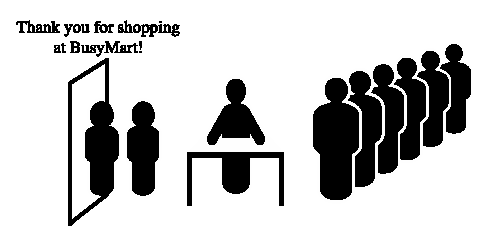
\epsfig{file=intro_figs/busy_mart.eps}
\caption{Customers waiting in line at BusyMart.}
\label{fig:busy_mart}
\end{figure}

To simulate this system, we will need an object to represent each customer in the line. 
A \classname{Customer} class is created for this purpose.
Customer objects have three attributes.
One attribute is the time needed to
ring up the customer's bill. Since we want to be able to determine
how long a customer has been waiting in line, we will also include
two attributes that record the time at which the customer entered the
queue and the time that the customer left the queue. The difference of these times is the amount of time that the customer spent waiting in line.
Here is the customer class, from which we will create customer
objects as needed. The class is coded in a single header file,
Customer.h.
\begin{verbatim}
#include "adevs.h"
/// A Busy-Mart customer.
struct Customer
{
    /// Time needed for the clerk to process the customer
    double twait;
    /// Time that the customer entered and left the queue
    double tenter, tleave;
};
/// Create an abbreviation for the Clerk's input/output type.
typedef adevs::PortValue<Customer*> IO_Type;
\end{verbatim}

The model of the clerk is our first example of an atomic model. Fortunately, the clerk's behavior is very simple.
The clerk has a line of people waiting at her counter. When a
customer arrives at the clerk's counter, that person is placed at the
end of the line. If the clerk is not busy and somebody is waiting
in line then the clerk rings up that customer's bill and sends
the customer on his way. The clerk then looks for another customer
waiting in line. If there is a customer, the clerk proceeds as
before. Otherwise, the clerk sits idly at her counter waiting for
more customers.

The DEVS model of the clerk is described in a particular way.
First, we need to specify the type of object that the clerk can consume and
produce. For this model, we use \classname{PortValue} objects. The \classname{PortValue}
class is part of the \classname{Digraph} model class, which will be introduced later. The \classname{PortValue} class describes a port/value pair.
Suppose that customers arrive in
line via an ``arrive" port and leave via a ``depart"
port and the value objects are instances of the \classname{Customer} class. 

The second thing that we need to determine are the state
variables that describe the clerk. In this case, 
we need to know which customers are in line. This can be
described with a list of customers; we can use a \classname{list} from the C++
Standard Template Library.

To complete the
model of the clerk, we must implement four methods that model the
clerk's behavior. First, let's construct the header
file for the clerk. Then we can proceed to fill in the details.
\begin{verbatim}
#include "adevs.h"
#include "Customer.h"
#include <list>
/**
 * The Clerk class is derived from the adevs Atomic class.
 * The Clerk's input/output type is specified using the template
 * parameter of the base class.
 */
class Clerk: public adevs::Atomic<IO_Type> 
{
    public:
        /// Constructor.
        Clerk();
        /// Internal transition function.
        void delta_int();
        /// External transition function.
        void delta_ext(double e, const adevs::Bag<IO_Type>& xb);
        /// Confluent transition function.
        void delta_conf(const adevs::Bag<IO_Type>& xb);
        /// Output function.  
        void output_func(adevs::Bag<IO_Type>& yb);
        /// Time advance function.
        double ta();
        /// Output value garbage collection.
        void gc_output(adevs::Bag<IO_Type>& g);
        /// Destructor.
        ~Clerk();
        /// Model input port.
        static const int arrive;
        /// Model output port.
        static const int depart;
    private:
        /// The clerk's clock
        double t;
        /// List of waiting customers.
        std::list<Customer*> line;
        /// Time spent so far on the customer at the front of the line
        double t_spent;
};
\end{verbatim}
This header file is a template for almost any atomic model that
we want to create. The \classname{Clerk} class is derived from the \adevs\ \classname{Atomic} class,
and it defines the virtual state transition,
output, time advance, and garbage collection methods that are required by the
\classname{Atomic} base class. The \classname{Clerk} also includes a set of static, constant
port variables that correspond to the \classname{Clerk}'s input (customer arrival) and
output (customer departure) ports. 

The constructor for the \classname{Clerk} class invokes
the constructor of the \classname{Atomic} base class. The template argument of the base
class is used to define the \classname{Clerk}'s input/output type. The \classname{Clerk} state variables
are defined as private class attributes.
The variables arrive and depart are assigned integer values that are unique within the scope of the \classname{Clerk} class.
Typically, the ports for a model are numbered in a way
that corresponds with the order in which they are listed; for example, 
\begin{verbatim}
// Assign locally unique identifiers to the ports
const int Clerk::arrive = 0;
const int Clerk::depart = 1;
\end{verbatim}

The \classname{Clerk} constructor 
places the \classname{Clerk} into its initial state.
For our experiment, this state is an empty line and the \classname{Clerk}'s clock
is initialized to zero.
\begin{verbatim}
Clerk::Clerk():
Atomic<IO_Type>(), // Initialize the parent Atomic model
t(0.0), // Set the clock to zero
t_spent(0.0) // No time spent on a customer so far
{
}
\end{verbatim}

Because the clerk has an empty line at first, the only interesting
thing that can happen is for a customer arrive. Customer arrivals
are events that appear on the clerk's ``arrive" input
port. The arrival of a customer will cause the clerk's external
transition method to be activated. The arguments to the method are
the time that has elapsed since the clerk last changed state and a
bag of \classname{PortValue} objects. 

The clerk's local clock is updated by adding the elapsed time to the current value of the clock. Next, the time spent working on the current customer's order is updated by adding the elapsed time to the time spent so far. After doing this, the input events are processed. Each \classname{PortValue} object has two fields.
The first is the port field; it contains the number of the port that the
event arrived on. The second is the \classname{Customer} that arrived.
The arrival time of every arriving customer is recorded and then the customer is placed
at the back of the line.
\begin{verbatim}
void Clerk::delta_ext(double e, const Bag<IO_Type>& xb)
{
    // Print a notice of the external transition
    cout << "Clerk: Computed the external transition function at t = " << t+e << endl;
    // Update the clock
    t += e;
    // Update the time spent on the customer at the front of the line
    if (!line.empty())
    {
        t_spent += e;
    }
    // Add the new customers to the back of the line.
    Bag<IO_Type>::const_iterator i = xb.begin();
    for (; i != xb.end(); i++)
    {
        // Copy the incoming Customer and place it at the back of the line.
        line.push_back(new Customer(*((*i).value)));
        // Record the time at which the customer entered the line.
        line.back()->tenter = t;
    }
    // Summarize the model state
    cout << "Clerk: There are " << line.size() << " customers waiting." << endl;
    cout << "Clerk: The next customer will leave at t = " << t+ta() << "." << endl;
}
\end{verbatim}

The time advance function gives the time at which the clerk will finish processing its current customer.  The time advance function describes the amount of time that should elapsed before the clerk's next internal (or self) event, barring an input that arrives in the interim.  The clerk's time advance function is very simple. If there are no customers in line, then the clerk will not do anything in the abscence of input, and so the time advance function returns infinity (here, represented by DBL\_MAX). Otherwise, the clerk will wait until the first customer has been rung up; i.e., until the difference of the \classname{Customer}'s twait and t\_spent has elapsed.
\begin{verbatim}
double Clerk::ta()
{
    // If the list is empty, then next event is at inf
    if (line.empty()) return DBL_MAX;
    // Otherwise, return the time remaining to process the current customer
    return line.front()->twait-t_spent;
}
\end{verbatim}

Eventually, the clerk will be done ringing up the customer. At this
time, the clerk sends the customer on his way and looks for a new
customer in the line. If there is another customer waiting in line,
the clerk will begin ringing that customer up in the same fashion as
before. This will all occur when the simulation clock
reaches the clerk's time of next event; i.e., the time of the clerk's last event plus the time advance. 

Two things happen when the time advance expires.
First, the \classname{Clerk}'s output method is called. When this
happens, the \classname{Clerk} places the departing customer on its
``depart" output port. Next, the \classname{Clerk}'s internal
transition method is activated. The \classname{Clerk}'s internal transition
method changes the state of the \classname{Clerk} by removing the departed
customer from the line.
The output function and
internal transition function are shown below.
\begin{verbatim}
void Clerk::delta_int()
{
    // Print a notice of the internal transition
    cout << "Clerk: Computed the internal transition function at t = " << t+ta() << endl;
    // Update the clock
    t += ta();
    // Reset the spent time 
    t_spent = 0.0;
    // Remove the departing customer from the front of the line.
    line.pop_front();
    // Summarize the model state
    cout << "Clerk: There are " << line.size() << " customers waiting." << endl;
    cout << "Clerk: The next customer will leave at t = " << t+ta() << "." << endl;
}
\end{verbatim}
\begin{verbatim}
void Clerk::output_func(Bag<IO_Type>& yb)
{
    // Get the departing customer
    Customer* leaving = line.front();
    // Set the departure time
    leaving->tleave = t + ta();
    // Eject the customer 
    IO_Type y(depart,leaving);
    yb.insert(y);
    // Print a notice of the departure
    cout << "Clerk: Computed the output function at t = " << t+ta() << endl;
    cout << "Clerk: A customer just departed!" << endl;
}
\end{verbatim}

At this point we have almost completely defined the behavior of the
model clerk; only one thing remains to be done. Suppose that a
customer arrives at the clerk's line at the same time that the clerk
has finished ringing up a customer. In this case we have a conflict
because the internal transition function and external transition
function must both be activated to handle these two events (i.e., the simultaneous arriving customer and departing customer).
These types of conflicts are resolved by the confluent transition
function. For the clerk model, the confluent transition function is
computed using the internal transition function first (to remove
the newly departed customer from the list) followed by the external
transition function (to add new customers to the end of the list and
begin ringing up the first customer). Below is the implementation of
the clerk's confluent transition function.
\begin{verbatim}
void Clerk::delta_conf(const Bag<IO_Type>& xb)
{
    delta_int();
    delta_ext(0.0,xb);
}
\end{verbatim}

To see how this model behaves, suppose we had customers arrive
according to the schedule shown in the table below.
\begin{table}
\centering
\begin{tabular}{|c|c|}
\hline
Enter checkout line & Time to process order \\ \hline
1 & 1 \\ \hline
2 & 4 \\ \hline
3 & 4 \\ \hline
5 & 2 \\ \hline
7 & 10 \\ \hline
8 & 20 \\ \hline
10 & 2 \\ \hline
11 & 1 \\ \hline
\end{tabular}
\caption{Customer arrival times and time to process customer orders.}
\label{tab:customer_data}
\end{table}
In this example, the first customer appears on the clerk's
``arrive" port at time 1, the next customer appears on the
``arrive" port at time 2, and so on. The print
statements in the \classname{Clerk}'s internal, external, and output
functions let us watch the evolution of the
clerk's line. Here is the output trace produced by the above sequence
of inputs.
\begin{verbatim}
Clerk: Computed the external transition function at t = 1
Clerk: There are 1 customers waiting.
Clerk: The next customer will leave at t = 2.
Clerk: Computed the output function at t = 2
Clerk: A customer just departed!
Clerk: Computed the internal transition function at t = 2
Clerk: There are 0 customers waiting.
Clerk: The next customer will leave at t = 1.79769e+308.
Clerk: Computed the external transition function at t = 2
Clerk: There are 1 customers waiting.
Clerk: The next customer will leave at t = 6.
Clerk: Computed the external transition function at t = 3
Clerk: There are 2 customers waiting.
Clerk: The next customer will leave at t = 6.
Clerk: Computed the external transition function at t = 5
Clerk: There are 3 customers waiting.
Clerk: The next customer will leave at t = 6.
Clerk: Computed the output function at t = 6
Clerk: A customer just departed!
Clerk: Computed the internal transition function at t = 6
Clerk: There are 2 customers waiting.
Clerk: The next customer will leave at t = 10.
Clerk: Computed the external transition function at t = 7
Clerk: There are 3 customers waiting.
Clerk: The next customer will leave at t = 10.
Clerk: Computed the external transition function at t = 8
Clerk: There are 4 customers waiting.
Clerk: The next customer will leave at t = 10.
Clerk: Computed the output function at t = 10
Clerk: A customer just departed!
Clerk: Computed the internal transition function at t = 10
Clerk: There are 3 customers waiting.
Clerk: The next customer will leave at t = 12.
Clerk: Computed the external transition function at t = 10
Clerk: There are 4 customers waiting.
Clerk: The next customer will leave at t = 12.
Clerk: Computed the external transition function at t = 11
Clerk: There are 5 customers waiting.
Clerk: The next customer will leave at t = 12.
Clerk: Computed the output function at t = 12
Clerk: A customer just departed!
Clerk: Computed the internal transition function at t = 12
Clerk: There are 4 customers waiting.
Clerk: The next customer will leave at t = 22.
Clerk: Computed the output function at t = 22
Clerk: A customer just departed!
Clerk: Computed the internal transition function at t = 22
Clerk: There are 3 customers waiting.
Clerk: The next customer will leave at t = 42.
Clerk: Computed the output function at t = 42
Clerk: A customer just departed!
Clerk: Computed the internal transition function at t = 42
Clerk: There are 2 customers waiting.
Clerk: The next customer will leave at t = 44.
Clerk: Computed the output function at t = 44
Clerk: A customer just departed!
Clerk: Computed the internal transition function at t = 44
Clerk: There are 1 customers waiting.
Clerk: The next customer will leave at t = 45.
Clerk: Computed the output function at t = 45
Clerk: A customer just departed!
Clerk: Computed the internal transition function at t = 45
Clerk: There are 0 customers waiting.
Clerk: The next customer will leave at t = 1.79769e+308.
\end{verbatim}

The basic simulation algorithm is illustrated by this example. Notice
that the external transition function is always activated when an
input (in this case, a customer) arrives on an input port. This is
because the external transition function describes the response of
the model to input events. 

The internal transition function is always
activated when the simulation clock has reached the model's time of
next event. The internal transition function describes the autonomous
behavior of the system (i.e., how the system responds to events that
it has scheduled for itself). Internal transitions are scheduled with
the time advance function.

The internal transition function is
always immediately preceded by the output function. Consequently, a
model can only produce outputs by scheduling an event for itself. The
value of the output is computed using the current state of the model.

To complete our simulation of the convenience store, we need two
other \classname{Atomic} models. The first model produce customers for the
\classname{Clerk} to serve. The customer arrival rate could be modeled using a
random variable with appropriate statistics, or
it could be driven by a table of values such as the one used in the
previous example. In either case, we hope that the customer arrival
process accurately reflects what happens in a typical day at the
convenience store. For this example, we will use a table to drive the
customer arrival process. Data for this table could come directly
from observing customers at the store, or it might be produced by a
statistical model in another tool (e.g., a spreadsheet program). 

We will use an \classname{Atomic} model called a \classname{Generator} to create customer
arrival events. The input file format is identical to that used
in the previous example. The input file contains a line for each
customer that arrives. Each line has the customer arrival time first,
followed by the customer service time. The \classname{Generator} is an input free
\classname{Atomic} model since all of its events are scripted in the input file.
The \classname{Generator} will need a single output port, which we will call
``arrive", through which is can export arriving customers.
The model state is the list of \classname{Customer}s that will arrive at the store.
Here is the header file for the
\classname{Generator}.
\begin{verbatim}
#include "adevs.h"
#include "Customer.h"
#include <list>
/**
 * This class produces Customers according to the provided schedule.
 */
class Generator: public adevs::Atomic<IO_Type> 
{
    public:
        /// Constructor.
        Generator(const char* data_file);
        /// Internal transition function.
        void delta_int();
        /// External transition function.
        void delta_ext(double e, const adevs::Bag<IO_Type>& xb);
        /// Confluent transition function.
        void delta_conf(const adevs::Bag<IO_Type>& xb);
        /// Output function.  
        void output_func(adevs::Bag<IO_Type>& yb);
        /// Time advance function.
        double ta();
        /// Output value garbage collection.
        void gc_output(adevs::Bag<IO_Type>& g);
        /// Destructor.
        ~Generator();
        /// Model output port.
        static const int arrive;

    private:    
        /// List of arriving customers.
        std::list<Customer*> arrivals;
}; 
\end{verbatim}

The dynamic behavior of this model is very simple. The constructor
opens the file containing the customer data and uses it
to create a list of \classname{Customer} objects. The inter-arrival times of the customers
are stored in their tenter fields. Here is the constuctor that initializes the model.
\begin{verbatim}
// Assign a locally unique number to the arrival port
const int Generator::arrive = 0;

Generator::Generator(const char* sched_file):
Atomic<IO_Type>()
{
    // Open the file containing the schedule
    fstream input_strm(sched_file);
    // Store the arrivals in a list
    double next_arrival_time = 0.0;
    double last_arrival_time = 0.0;
    while (true)
    {
        Customer* customer = new Customer;
        input_strm >> next_arrival_time >> customer->twait;
        // Check for end of file
        if (input_strm.eof())
        {
            delete customer;
            break;
        }
        // The entry time holds the inter arrival times, not the
        // absolute entry time.
        customer->tenter = next_arrival_time-last_arrival_time;
        // Put the customer at the back of the line
        arrivals.push_back(customer);
        last_arrival_time = next_arrival_time;
    }
}
\end{verbatim}

Because the generator is input free, the external transition function
is empty. Similarly, the confluent transition function merely calls
the internal transition function. 
\begin{verbatim}
void Generator::delta_ext(double e, const Bag<IO_Type>& xb)
{
    /// The generator is input free, and so it ignores external events.
}

void Generator::delta_conf(const Bag<IO_Type>& xb)
{
    /// The generator is input free, and so it ignores input.
    delta_int();
}
\end{verbatim}

The effect of an internal event (i.e., an event scheduled for the
generator by itself) is to first place the arriving \classname{Customer} onto the
\classname{Generator}'s ``arrive" output port. This is done by the
output function.
\begin{verbatim}
void Generator::output_func(Bag<IO_Type>& yb)
{
    // First customer in the list is produced as output
    IO_Type output(arrive,arrivals.front());
    yb.insert(output);
}
\end{verbatim}
After the generator has produced this output event, its internal
transition function removes the newly arrived customer from the arrival list.
\begin{verbatim}
void Generator::delta_int()
{
    // Remove the first customer.  Because it was used as the
    // output object, it will be deleted during the gc_output()
    // method call at the end of the simulation cycle.
    arrivals.pop_front();
}
\end{verbatim}

Internal events are scheduled with the time advance function. The \classname{Generator}'s time advance function returns the time remaining until the next \classname{Customer} arrives at the store. Remember that the tarrival field contains \classname{Customer}'s the inter-arrival times, not the absolute arrival times.
\begin{verbatim}
double Generator::ta()
{
    // If there are not more customers, next event time is infinity
    if (arrivals.empty()) return DBL_MAX;
    // Otherwise, wait until the next arrival
    return arrivals.front()->tenter;
}
\end{verbatim}

To conduct the simulation experiment, the \classname{Generator} output is coupled to the \classname{Clerk} input.  By doing this,
\classname{Customer} objects apprearing on the \classname{Generator}'s 
``arrive" output port cause a
corresponding appearance of a \classname{Customer} on the \classname{Clerk}'s ``arrive" input port.
This input event, in turn, causes the \classname{Clerk}'s external
transition function to be activated. The relationship between input
and output events can be best understood by viewing the whole model as two
distinct components, the \classname{Generator} and the \classname{Clerk}, that are connected
via their input and output ports. This view of the model is depicted
in Figure \ref{fig:clerk_and_generator}.
\begin{figure}[ht]
\centering
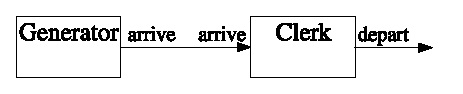
\epsfig{file=intro_figs/generator_and_clerk.eps}
\caption{The combined \classname{Generator} and \classname{Clerk} model.}
\label{fig:clerk_and_generator}
\end{figure}

As Figure \ref{fig:clerk_and_generator} suggests, output events produced by the \classname{Generator} on its ``arrive" port, via the output function, will appear
as input events on the \classname{Clerk}'s ``arrive" port when the \classname{Clerk}'s
external transition function is evaluated. The component models and
their interconnections constitute a coupled (or network) model. To
create the coupled model depicted above, we need to create an
instance of a \classname{Digraph} model that has the \classname{Generator} and \classname{Clerk} as
component models. Shown below is the code snippet that creates this two component model.
\begin{verbatim}
int main(int argc, char** argv)
{
    ...
    // Create a digraph model whose components use PortValue<Customer*>
    // objects as input and output objects.
    adevs::Digraph<Customer*> store;
    // Create and add the component models
    Clerk* clrk = new Clerk();
    Generator* genr = new Generator(argv[1]); 
    store.add(clrk);
    store.add(genr);
    // Couple the components
    store.couple(genr,genr->arrive,clrk,clrk->arrive);
    ...
\end{verbatim}
This code snippet first creates the components models and then adds them to
the \classname{Digraph}.
Next, the components are
interconnected by coupling the ``arrive" output port of
the \classname{Generator} to the ``arrive" input port of the
\classname{Clerk}.

Having created a coupled model which represents the
store, all that remains is to perform the simulation. Here is the
code necessary to simulate our model.
\begin{verbatim}
adevs::Simulator<IO_Type> sim(&store);
while (sim.nextEventTime() < DBL_MAX)
{
    sim.execNextEvent();
}
\end{verbatim}

Putting this all of this together gives the main routine for the simulation
program that will generate the execution traces that are shown in the
above examples.
\begin{verbatim}
#include "Clerk.h"
#include "Generator.h"
#include "Observer.h"
#include <iostream>
using namespace std;

int main(int argc, char** argv)
{
    if (argc != 3)
    {
        cout << "Need input and output files!" << endl;
        return 1;
    }
    // Create a digraph model whose components use PortValue<Customer*>
    // objects as input and output objects.
    adevs::Digraph<Customer*> store;
    // Create and add the component models
    Clerk* clrk = new Clerk();
    Generator* genr = new Generator(argv[1]);
    Observer* obsrv = new Observer(argv[2]);
    store.add(clrk);
    store.add(genr);
    store.add(obsrv);
    // Couple the components
    store.couple(genr,genr->arrive,clrk,clrk->arrive);
    store.couple(clrk,clrk->depart,obsrv,obsrv->departed);
    // Create a simulator and run until its done
    adevs::Simulator<IO_Type> sim(&store);
    while (sim.nextEventTime() < DBL_MAX)
    {
        sim.execNextEvent();
    }
    // Done, component models are deleted when the Digraph is
    // deleted.
    return 0;
}
\end{verbatim}

We have completed our first \adevs\ simulation program! However, a few
details have been glossed over. The first question, an
essential one for a programming language without garbage collection,
is what happens to the objects that we created in the \classname{Generator} and \classname{Clerk} output functions?

The answer is that each model has a
garbage collection method that is called at the end of every
simulation cycle. The argument to the garbage collection method is
the bag of objects created as output in the current
simulation cycle. In our store example, the \classname{Atomic} models simply
delete the customer pointed to by each \classname{PortValue} object in the
garbage list. The implementation of the garbage collection method is
shown below. This listing is for the \classname{Generator} model; the \classname{Clerk}'s
\methodname{gc\_output()} method is identical.
\begin{verbatim}
void Generator::gc_output(Bag<IO_Type>& g)
{
    // Delete the customer that was produced as output
    Bag<IO_Type>::iterator i;
    for (i = g.begin(); i != g.end(); i++)
    {
        delete (*i).value;
    }
}
\end{verbatim}

A second issue that has been overlooked is how to collect the
statistics that were our original objective. One approach is to
modify the \classname{Clerk} so that it writes waiting times to a file as
\classname{Customer}s are processed. While this could work, it has the
unfortunate effect of cluttering up the \classname{Clerk} with experiment
specific code. 

A better approach is to have an \classname{Observer} that is
coupled to the \classname{Clerk}'s ``depart" output port. The
\classname{Observer} can record the desired statistics as it receives \classname{Customer}s
on its ``depart" input port. The advantage of this
approach is that we can modify the \classname{Clerk} model to perform the same
experiment on different queueing strategies (e.g., we could add a
priority to each customer and have the clerk process customers
with a high priority first) without changing the experimental
setup (i.e., customer generation and data collection). We can also
change the experiment (i.e., customer generation and data collection)
without changing the clerk.

Below is a listing of the \classname{Observer} class. The model is driven
solely by external events. The effect of an external event is simply
to have the model record the time that the \classname{Customer} departed the
\classname{Clerk}'s queue (i.e., the current simulation time) and the amount of time that
the \classname{Customer} waited in line. Here is the \classname{Observer} header file.
\begin{verbatim}
#include "adevs.h"
#include "Customer.h"
#include <fstream>
/**
 * The Observer records performance statistics for a Clerk model
 * based on its observable output.
 */
class Observer: public adevs::Atomic<IO_Type>
{
    public:
        /// Input port for receiving customers that leave the store.
        static const int departed;
        /// Constructor. Results are written to the specified file.
        Observer(const char* results_file);
        /// Internal transition function.
        void delta_int();
        /// External transition function.
        void delta_ext(double e, const adevs::Bag<IO_Type>& xb);
        /// Confluent transition function.
        void delta_conf(const adevs::Bag<IO_Type>& xb);
        /// Time advance function.
        double ta();
        /// Output function.  
        void output_func(adevs::Bag<IO_Type>& yb);
        /// Output value garbage collection.
        void gc_output(adevs::Bag<IO_Type>& g);
        /// Destructor.
        ~Observer();
    private:    
        /// File for storing information about departing customers.
        std::ofstream output_strm;
}; 
\end{verbatim}
Below is the \classname{Observer} source file.
\begin{verbatim}
#include "Observer.h"
using namespace std;
using namespace adevs;

// Assign a locally unique number to the input port
const int Observer::departed = 0;

Observer::Observer(const char* output_file):
Atomic<IO_Type>(),
output_strm(output_file)
{
    // Write a header describing the data fields
    output_strm << "# Col 1: Time customer enters the line" << endl;
    output_strm << "# Col 2: Time required for customer checkout" << endl;
    output_strm << "# Col 3: Time customer leaves the store" << endl;
    output_strm << "# Col 4: Time spent waiting in line" << endl;
}

double Observer::ta()
{
    // The Observer has no autonomous behavior, so its next event
    // time is always infinity.
    return DBL_MAX;
}

void Observer::delta_int()
{
    // The Observer has no autonomous behavior, so do nothing
}

void Observer::delta_ext(double e, const Bag<IO_Type>& xb)
{
    // Record the times at which the customer left the line and the
    // time spent in it.
    Bag<IO_Type>::const_iterator i;
    for (i = xb.begin(); i != xb.end(); i++)
    {
        const Customer* c = (*i).value;
        // Compute the time spent waiting in line 
        double waiting_time = (c->tleave-c->tenter)-c->twait;
        // Dump stats to a file
        output_strm << c->tenter << " " << c->twait << " " << c->tleave << " " << waiting_time << endl;
    }
}

void Observer::delta_conf(const Bag<IO_Type>& xb)
{
    // The Observer has no autonomous behavior, so do nothing
}

void Observer::output_func(Bag<IO_Type>& yb)
{
    // The Observer produces no output, so do nothing
}

void Observer::gc_output(Bag<IO_Type>& g)
{
    // The Observer produces no output, so do nothing
}

Observer::~Observer()
{
    // Close the statistics file
    output_strm.close();
}
\end{verbatim}

This model is coupled to the \classname{Clerk}'s ``depart" output port in the same manner as before. The resulting coupled model is illustrated in Figure \ref{fig:complete_store_model};
now we have three components instead of just two.
\begin{figure}[ht]
\centering
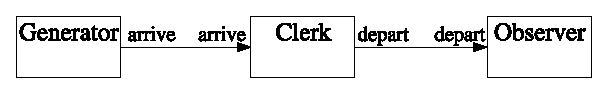
\epsfig{file=intro_figs/generator_and_clerk_and_observer.eps}
\caption{The \classname{Generator}, \classname{Clerk}, and \classname{Observer} model.} 
\label{fig:complete_store_model}
\end{figure}

Given the customer arrival data in Table \ref{tab:customer_data}, the corresponding customer depature and waiting times are
shown in Table \ref{tab:simulation_output}. Given this output, we could use a spreadsheet or
some other suitable software to find the maximum and average customer
wait times.
\begin{table}
\centering
\begin{tabular}{|c|c|}
\hline
Time that the customer leaves the store & Time spent waiting in line \\ \hline
2 & 0 \\ \hline
6 & 0 \\ \hline
10 & 3 \\ \hline
12 & 5 \\ \hline
22 & 5 \\ \hline
42 & 14 \\ \hline
44 & 32 \\ \hline
45 & 33 \\ \hline
\end{tabular}
\caption{Customer departure times and wait times.}
\label{tab:simulation_output}
\end{table}

Again, notice that the customer
depature times correspond exactly with the production of customer
depature events by the \classname{Clerk} model. These customer depature events
are delivered to the \classname{Observer} via the \classname{Clerk} to \classname{Observer}
coupling shown in Figure \ref{fig:complete_store_model}. Each entry in Table \ref{tab:simulation_output} is the result of
executing the \classname{Observer}'s external transition function.
Also notice that the \classname{Observer}'s internal and confluent transition functions will never be executed. This is because the
\classname{Observer}'s \methodname{ta()} method always returns infinity.

This section has demonstrated the most common parts of a simulation program that is built with \adevs. The remainder of the manual covers \classname{Atomic} and \classname{Network} models in greater detail, demonstrates the construction of variable structure models, and shows how continuous models can be added to your discrete event simulation.
